\documentclass{standalone}

\usepackage{tikz,tikzpeople}
\usetikzlibrary{arrows.meta,matrix,backgrounds,fit,shapes,positioning}


\begin{document}
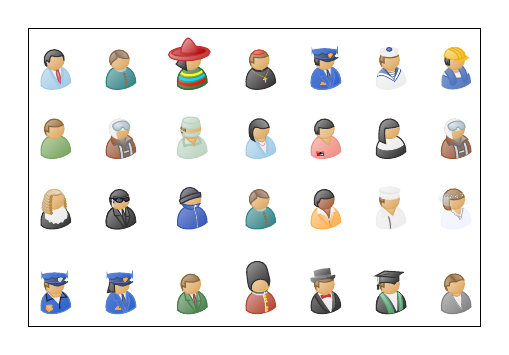
\begin{tikzpicture}
   \tikzstyle{sel}=[draw]
   \tikzstyle{pn}=[outer sep=3mm]
   \tikzstyle{ar}=[gray!50,->]
   \tikzstyle{sel}=[rectangle,fill=yellow!10]
   \tikzstyle{head}=[text=blue]

   \matrix (pop) [draw,matrix of nodes,row sep=3mm,column sep=4mm] {
      \node [pn,dave] {} ; &
      \node [pn,charlie] {} ; &
      \node [pn,mexican] {} ; &
      \node [pn,priest] {} ; &
      \node [pn,conductor] {} ; &
      \node [pn,sailor] {} ; &
      \node (p2) [pn,builder] {} ; \\
      \node [pn,person] {} ; &
      \node [pn,pilot,female] {} ; &
      \node [pn,surgeon] {} ; &
      \node [pn,dave,female] {} ; &
      \node (p1) [pn,nurse] {} ; &
      \node [pn,nun] {} ; &
      \node [pn,pilot] {} ; \\
      \node [pn,judge] {} ; &
      \node [pn,maninblack] {} ; &
      \node [pn,criminal] {} ; &
      \node [pn,charlie] {} ; &
      \node [pn,alice] {} ; &
      \node (p4) [pn,chef] {} ; &
      \node [pn,bride] {} ; \\
      \node [pn,police] {} ; &
      \node [pn,conductor,female] {} ; &
      \node [pn,businessman] {} ; &
      \node [pn,guard] {} ; &
      \node (p3) [pn,groom] {} ; &
      \node [pn,graduate] {} ; &
      \node [pn,bob] {} ; \\
   } ;
\end{tikzpicture}
\end{document}
